\section{Overall Description}

\subsection{User needs}

\begin{content}
ECAP5 is the primary user for ECAP5-DPROC. ECAP5-DPROC could however be used as a standalone RISC-V processor. The following requirements define the user needs. 
\end{content}

\ureq{U\_INSTRUCTION\_SET\_01}{
  ECAP5-DPROC shall implement the RV32I instruction set.
}

\begin{content}
  In order to improve the usability of ECAP5-DPROC, it shall have a \textit{von Neumann} architecture as it only requires one memory interface.
\end{content}

\ureq{U\_MEMORY\_INTERFACE\_01}{
  ECAP5-DPROC shall access both instructions and data through a unique memory interface.
}

\ureq{U\_MEMORY\_INTERFACE\_02}{
  ECAP5-DPROC's unique memory interface shall be compliant with the AXI-Lite specification.
}

\ureq{U\_RESET\_01}{
  ECAP5-DPROC shall provide a signal which shall hold ECAP5-DPROC in a reset state while asserted.
}

\begin{content}
The polarity of the reset signal mentionned in \texttt{U\_RESET\_01} is not specified by the user.
\end{content}

\ureq{U\_BOOT\_ADDRESS\_01}{
  The address at which ECAP5-DPROC jumps after the reset signal is deasserted shall be hardware-configurable.
}

\begin{content}
The address mentionned in \texttt{U\_BOOT\_ADDRESS\_01} can be either configured through hardware signals or can be selected at compile-time.
\end{content}

\ureq{U\_HARDWARE\_INTERRUPT\_01}{
  ECAP5-DPROC shall provide an signal which shall interrupt ECAP5-DPROC's execution flow while asserted.
}

\ureq{U\_HARDWARE\_INTERRUPT\_02}{
  ECAP5-DPROC shall jump to a software-configurable address when it is interrupted.
}

\begin{content}
The memory address at which ECAP5-DPROC shall jump to when interrupted is not specified by the user.
\end{content}

\ureq{U\_DEBUG\_01}{
  ECAP5-DPROC shall be compliant with the RISC-V External Debug Support specification.
}

\begin{content}
There is no performance goal required by ECAP5 for ECAP5-DPROC as ECAP5 is an educational platform.
\end{content}

\subsection{Assumptions and Dependencies}

\begin{content}
Describe what the assumptions for the product are : Targeting the ecp5 family, based around opensource toolchains.
\end{content}

\section{Requirements}

\subsection{External Interface Requirements}

\begin{figure}[h!]
    \centering
    \scalebox{0.85}{
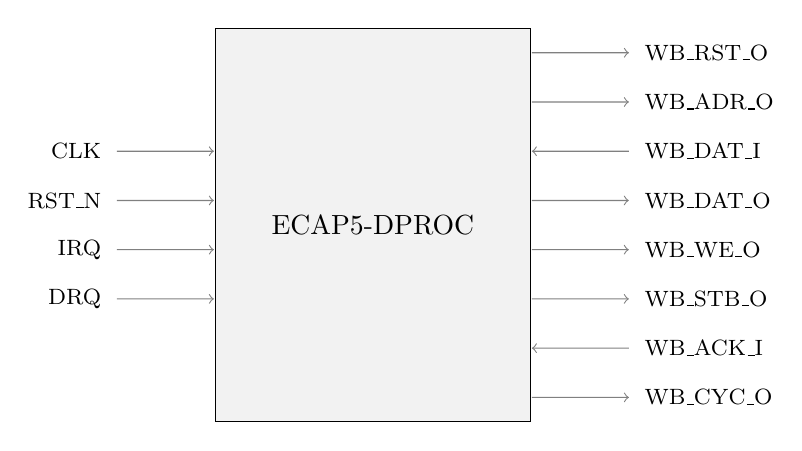
\begin{tikzpicture}[scale=1.25, draw=gray, inner sep=0, outer sep=0]
  \node[rectangle, draw=black,
    minimum height = 5cm,
    minimum width = 4cm,
    fill = gray!10] (box) at (0, 0) {ECAP5-DPROC};

  % left
  \node (lport1) at ([yshift=0.75cm]box.west) {};
  \node (lport2) at ([yshift=0.25cm]box.west) {};
  \node (lport3) at ([yshift=-0.25cm]box.west) {};
  \node (lport4) at ([yshift=-0.75cm]box.west) {};

  \draw[->] ([xshift=-1cm]lport1.center) node[left=0.2cm, anchor=east]{\footnotesize CLK} -- (lport1);
  \draw[->] ([xshift=-1cm]lport2.center) node[left=0.2cm, anchor=east]{\footnotesize RST\_N} -- (lport2);
  \draw[->] ([xshift=-1cm]lport3.center) node[left=0.2cm, anchor=east]{\footnotesize IRQ} -- (lport3);
  \draw[->] ([xshift=-1cm]lport4.center) node[left=0.2cm, anchor=east]{\footnotesize DRQ} -- (lport4);

  % right
  \node (rport4) at ([yshift=0.25cm]box.east) {};
  \node (rport3) at ([yshift=0.5cm]rport4.center) {};
  \node (rport2) at ([yshift=0.5cm]rport3.center) {};
  \node (rport1) at ([yshift=0.5cm]rport2.center) {};

  \node (rport5) at ([yshift=-0.25cm]box.east) {};
  \node (rport6) at ([yshift=-0.5cm]rport5.center) {};
  \node (rport7) at ([yshift=-0.5cm]rport6.center) {};
  \node (rport8) at ([yshift=-0.5cm]rport7.center) {};

  \draw[<-] ([xshift=1cm]rport1.center) node[right=0.2cm, anchor=west]{\footnotesize WB\_RST\_O} -- (rport1);
  \draw[<-] ([xshift=1cm]rport2.center) node[right=0.2cm, anchor=west]{\footnotesize WB\_ADR\_O} -- (rport2);
  \draw[->] ([xshift=1cm]rport3.center) node[right=0.2cm, anchor=west]{\footnotesize WB\_DAT\_I} -- (rport3);
  \draw[<-] ([xshift=1cm]rport4.center) node[right=0.2cm, anchor=west]{\footnotesize WB\_DAT\_O} -- (rport4);
  \draw[<-] ([xshift=1cm]rport5.center) node[right=0.2cm, anchor=west]{\footnotesize WB\_WE\_O} -- (rport5);
  \draw[<-] ([xshift=1cm]rport6.center) node[right=0.2cm, anchor=west]{\footnotesize WB\_STB\_O} -- (rport6);
  \draw[->] ([xshift=1cm]rport7.center) node[right=0.2cm, anchor=west]{\footnotesize WB\_ACK\_I} -- (rport7);
  \draw[<-] ([xshift=1cm]rport8.center) node[right=0.2cm, anchor=west]{\footnotesize WB\_CYC\_O} -- (rport8);
\end{tikzpicture}
}

    \caption{Schematic view of the external interface of ECAP5-DPROC}
    \label{fig:externalinterface}
\end{figure}

\begin{table}[H]
  \centering
  {
\footnotesize
\begin{tabularx}{0.9\textwidth}{|l|c|c|X|}
  \hline
  \cellcolor{gray!20}\textbf{NAME} & \cellcolor{gray!20}\textbf{TYPE} & \cellcolor{gray!20}\textbf{WIDTH} & \cellcolor{gray!20}\textbf{DESCRIPTION} \\
  \hline
  CLK & I & 1 & Clock input. \\
  \hline
  RST\_N & I & 1 & Hardware reset. Active low. \\
  \hline
  IRQ & I & 1 & External interrupt request. \\
  \hline
  DRQ & I & 1 & Debug request. \\
  \hline
\end{tabularx}
}

  \caption{ECAP5-DPROC control signals}
  \label{tab:control-interface}
\end{table}

\begin{table}[H]
  \centering
  {
\footnotesize
\begin{tabularx}{0.9\textwidth}{|l|c|c|X|}
  \hline
  \cellcolor{gray!20}\textbf{NAME} & \cellcolor{gray!20}\textbf{TYPE} & \cellcolor{gray!20}\textbf{WIDTH} & \cellcolor{gray!20}\textbf{DESCRIPTION} \\
  \hline
  \multicolumn{4}{|l|}{\textbf{READ ADDRESS BUS}} \\
  \hline
  ARADDR & O & 32 & Read address. \\
  \hline
  ARVALID & O & 1 & Read address valid. \\
  \hline
  ARREADY & I & 1 & Read address ready. \\ 
  \hline
  \multicolumn{4}{|l|}{\textbf{READ DATA BUS}} \\
  \hline
  RDATA & I & 32 & Read data. \\
  \hline
  RRESP & I & 2 & Read response. \\
  \hline
  RVALID & I & 1 & Read valid. \\
  \hline
  RREADY & O & 1 & Read ready. \\ 
  \hline
  \multicolumn{4}{|l|}{\textbf{WRITE ADDRESS BUS}} \\
  \hline
  AWADDR & O & 32 & Write address. \\
  \hline
  AWVALID & O & 1 & Write address valid. \\
  \hline
  AWREADY & I & 1 & Write address ready \\
  \hline
  \multicolumn{4}{|l|}{\textbf{WRITE DATA BUS}} \\
  \hline
  WDATA & O & 32 & Write data. \\
  \hline
  WSTRB & O & 4 & Write strobes. \\
  \hline
  \multicolumn{4}{|l|}{\textbf{WRITE RESPONSE BUS}} \\
  \hline
  BRESP & I & 2 & Write response. \\
  \hline
  BVALID & I & 1 & Write response valid. \\
  \hline
  BREADY & O & 1 & Response ready. \\
  \hline
\end{tabularx}
}

  \caption{ECAP5-DPROC memory interface signals}
  \label{tab:memory-interface}
\end{table}

\ireq{I\_CLK\_01}{
  All inputs and outputs of ECAP5-DPROC shall belong to CLK's clock domain.
}{}

\ireq{I\_RESET\_01}{
  The RST\_N signal shall hold ECAP5-DPROC in a reset state while asserted.
}{
  U\_RESET\_01
}

\ireq{I\_RESET\_02}{
  RST\_N polarity shall be active low.
}{}

\ireq{I\_IRQ\_01}{
  ECAP5-DPROC shall jump to a software-configurable address when input IRQ is asserted.
}{
  U\_HARDWARE\_INTERRUPT\_01, U\_HARDWARE\_INTERRUPT\_02
}

\ireq{I\_DIRQ\_01}{
  TBD
}{}

\ireq{I\_MEMORY\_INTERFACE\_01}{
  Signals from table \ref{tab:memory-interface} shall be compliant with the AXI-Lite specification.
}{
  U\_MEMORY\_INTERFACE\_02
}

\begin{content}
  Behavioral specification for symbols in table \ref{tab:memory-interface} is outlined in the functional requirements section, subsection \ref{spec-memory-interface}.
\end{content}

\subsection{Functional Requirements}

\subsubsection{Register file}

\req{F\_REGISTERS\_01}{
  ECAP5-DPROC shall implement 31 user-accessible general purpose registers ranging from \texttt{x0} to \texttt{x31}.
}{U\_INSTRUCTION\_SET\_01}

\req{F\_REGISTERS\_02}{
  Register \texttt{x0} shall be hardwired to the constant zero.
}{U\_INSTRUCTION\_SET\_01}

\req{F\_REGISTERS\_03}{
  ECAP5-DPROC shall implement a \texttt{pc} user-accessible register storing the address of the current instruction.
}{U\_INSTRUCTION\_SET\_01}

\subsubsection{Instruction decoding}

\begin{content}
  Figure \ref{fig:instructionencoding} outlines the different instruction encodings for the RV32I instruction set. The \texttt{opcode} parameter is a unique identifier for each instruction. The instruction encoding is infered from the opcode as there can only be one encoding per opcode.
\end{content}

\begin{figure}[h!]
    \centering
    \vspace{0.5em}

\hspace{2em}
\scalebox{0.9}{
\begin{bytefield}[
    bitwidth=1.1em, 
    endianness=big, 
    bitformatting={\scriptsize}, 
    boxformatting={\centering\footnotesize\ttfamily},
    rightcurly=., rightcurlyspace=5pt
]{32}
  \bitheader{0,6,7,8,11,12,14,15,19,20,24,25,31} \\
  \begin{rightwordgroup}{\footnotesize R-type}
    \bitbox{7}{funct7}
    \bitbox{5}{rs2}
    \bitbox{5}{rs1}
    \bitbox{3}{func3}
    \bitbox{5}{rd}
    \bitbox{7}{opcode}
  \end{rightwordgroup}
  \\[2ex]
  \begin{rightwordgroup}{\footnotesize I-type}
    \bitbox{12}{imm[11:0]}
    \bitbox{5}{rs1}
    \bitbox{3}{func3}
    \bitbox{5}{rd}
    \bitbox{7}{opcode}
  \end{rightwordgroup}
  \\[2ex]
  \begin{rightwordgroup}{\footnotesize S-type}
    \bitbox{7}{imm[11:5]}
    \bitbox{5}{rs2}
    \bitbox{5}{rs1}
    \bitbox{3}{func3}
    \bitbox{5}{imm[4:0]}
    \bitbox{7}{opcode}
  \end{rightwordgroup}
  \\[2ex]
  \begin{rightwordgroup}{\footnotesize B-type}
    \bitbox{1}{a}
    \bitbox{6}{imm[10:5]}
    \bitbox{5}{rs2}
    \bitbox{5}{rs1}
    \bitbox{3}{func3}
    \bitbox{4}{imm[4:1]}
    \bitbox{1}{b}
    \bitbox{7}{opcode}
  \end{rightwordgroup}
  \\[2ex]
  \begin{rightwordgroup}{\footnotesize U-type}
    \bitbox{20}{imm[31:12]}
    \bitbox{5}{rd}
    \bitbox{7}{opcode}
  \end{rightwordgroup}
  \\[2ex]
  \begin{rightwordgroup}{\footnotesize J-type}
    \bitbox{1}{c}
    \bitbox{10}{imm[10:1]}
    \bitbox{1}{b}
    \bitbox{8}{imm[31:12]}
    \bitbox{5}{rd}
    \bitbox{7}{opcode}
  \end{rightwordgroup}
\end{bytefield}
}

\vspace{0.25em}
\scalebox{0.7}{
\begin{tabularx}{0.8\textwidth}{Y Y Y}
a: \texttt{imm[12]} & b: \texttt{imm[11]} & c: \texttt{imm[20]}
\end{tabularx}
}

    \caption{Instruction encodings of the RV32I instruction set}
    \label{fig:instructionencoding}
\end{figure}

\paragraph{Immediate encoding}

\begin{content}
  Only one immediate value can be encoded in one instruction. The value can be reconstructed from fragments of the following format : imm[x] representing the x\textsuperscript{th} bit or imm[x:y] representing bits from the x\textsuperscript{th} to the y\textsuperscript{th} both included.
\end{content}

\req{F\_INSTR\_IMMEDIATE\_01}{
  Immediate values shall be sign-extended.
}{U\_INSTRUCTION\_SET\_01}

\begin{content}
  RV32I is called a Load/Store ISA, meaning that instructions inputs and outputs are passed through registers or through an instruction immediate. There are specific instructions for loading and storing data into memory.
\end{content}

\paragraph{Instruction inputs}

\req{F\_INSTR\_FIRST\_INPUT\_01}{
  Instructions encoded using the R-type, I-type, S-type and B-type shall take as their first input the value stored in the register designated by the \texttt{rs1} parameter.
}{U\_INSTRUCTION\_SET\_01}

\req{F\_INSTR\_FIRST\_INPUT\_02}{
  Instructions encoded using the U-type and J-type shall take as their first input the immediate value encoded in the instruction.
}{U\_INSTRUCTION\_SET\_01}

\req{F\_INSTR\_SECOND\_INPUT\_01}{
  Instructions encoded using the R-type, S-type and B-type shall take as their second input the value stored in the register designated by the \texttt{rs2} parameter.
}{U\_INSTRUCTION\_SET\_01}

\req{F\_INSTR\_SECOND\_INPUT\_02}{
  Instructions encoded using the I-type shall take as its second input the immediate value encoded in the instruction.
}{U\_INSTRUCTION\_SET\_01}

\req{F\_INSTR\_THIRD\_INPUT\_01}{
  Instructions encoded using the S-type and B-type shall take as their third input the immediate value encoded in the instruction.
}{U\_INSTRUCTION\_SET\_01}

\paragraph{Instruction outputs}

\req{F\_INSTR\_OUTPUT\_01}{
  Instructions encoded using the R-type, I-type, U-type and J-type shall store their result in the register designated by the \texttt{rd} parameter.
}{U\_INSTRUCTION\_SET\_01}

\req{F\_INSTR\_OUTPUT\_02}{
  Instructions encoded using the S-type and B-type do not produce any result.
}{U\_INSTRUCTION\_SET\_01}

\paragraph{Instruction variants}

\req{F\_INSTR\_VARIANT\_01}{
  Instructions encoded using the R-type, I-type, S-type and B-type shall use the \texttt{func3} parameter as a behavior variant selector.
}{U\_INSTRUCTION\_SET\_01}

\req{F\_INSTR\_VARIANT\_02}{
  Instructions encoded using the R-type shall use the \texttt{func7} parameter as a secondary behavior variant selector.
}{U\_INSTRUCTION\_SET\_01}

\paragraph{Opcodes}

\vspace{1em}
\begin{content}
  Table \ref{tab:opcodemap} outlines the different opcodes values of the RV32I instruction set. Cells marked as \textit{noimp} are for opcodes that are not implemented in ECAP5-DPROC.
\end{content}

\begin{table}[H]
  \centering
  \scalebox{0.8}{
\footnotesize
\begin{tabular}{|r|c|c|c|c|c|c|c|c|}
  \hline
  opcode[1:0] & \multicolumn{8}{|c|}{11} \\
  \hline
  opcode[4:2] & \multirow{2}{*}{000} & \multirow{2}{*}{001} & \multirow{2}{*}{010} & \multirow{2}{*}{011} & \multirow{2}{*}{100} & \multirow{2}{*}{101} & \multirow{2}{*}{110} & \multirow{2}{*}{111} \\
  \cline{1-1}
  opcode[6:5] & & & & & & & & \\
  \hline
  00 & LOAD & \cellcolor{gray!20}\textit{noimp} & \cellcolor{gray!20}\textit{noimp} & MISC-MEM & OP-IMM & AUIPC & \cellcolor{gray!20}\textit{noimp} & \cellcolor{gray!20}\textit{noimp} \\
  \hline
  01 & STORE & \cellcolor{gray!20}\textit{noimp} & \cellcolor{gray!20}\textit{noimp} & \cellcolor{gray!20}\textit{noimp} & OP & LUI & \cellcolor{gray!20}\textit{noimp} & \cellcolor{gray!20}\textit{noimp} \\
  \hline
  10 & \cellcolor{gray!20}\textit{noimp} & \cellcolor{gray!20}\textit{noimp} & \cellcolor{gray!20}\textit{noimp} & \cellcolor{gray!20}\textit{noimp} & \cellcolor{gray!20}\textit{noimp} & \cellcolor{gray!20}\textit{noimp} & \cellcolor{gray!20}\textit{noimp} & \cellcolor{gray!20}\textit{noimp} \\
  \hline
  11 & BRANCH & JALR & \cellcolor{gray!20}\textit{noimp} & JAL & SYSTEM & \cellcolor{gray!20}\textit{noimp} & \cellcolor{gray!20}\textit{noimp} & \cellcolor{gray!20}\textit{noimp} \\
  \hline
\end{tabular}
}

  \caption{Opcode values for the RV32I instruction set.}
  \label{tab:opcodemap}
\end{table}

\req{F\_OPCODE\_ENCODING\_01}{
  Instructions which use the LUI opcode shall be decoded as an U-type instruction.
}{U\_INSTRUCTION\_SET\_01}

\req{F\_OPCODE\_ENCODING\_02}{
  Instructions which use the AUIPC opcode shall be decoded as an U-type instruction.
}{U\_INSTRUCTION\_SET\_01}

\req{F\_OPCODE\_ENCODING\_03}{
  Instructions which use the JAL opcode shall be decoded as a J-type instruction.
}{U\_INSTRUCTION\_SET\_01}

\req{F\_OPCODE\_ENCODING\_04}{
  Instructions which use the JALR opcode shall be decoded as an I-type instruction.
}{U\_INSTRUCTION\_SET\_01}

\req{F\_OPCODE\_ENCODING\_05}{
  Instructions which use the BRANCH opcode shall be decoded as a B-type instruction.
}{U\_INSTRUCTION\_SET\_01}

\req{F\_OPCODE\_ENCODING\_06}{
  Instructions which use the LOAD opcode shall be decoded as an I-type instruction.
}{U\_INSTRUCTION\_SET\_01}

\req{F\_OPCODE\_ENCODING\_07}{
  Instructions which use the STORE opcode shall be decoded as a S-type instruction.
}{U\_INSTRUCTION\_SET\_01}

\req{F\_OPCODE\_ENCODING\_08}{
  Instructions which use the OP-IMM opcode shall be decoded as an I-type instruction.
}{U\_INSTRUCTION\_SET\_01}

\req{F\_OPCODE\_ENCODING\_09}{
  Instructions which use the OP opcode shall be decoded as a R-type instruction.
}{U\_INSTRUCTION\_SET\_01}

\req{F\_OPCODE\_ENCODING\_10}{
  Instructions which use the MISC-MEM opcode shall be decoded as an I-type instruction.
}{U\_INSTRUCTION\_SET\_01}

\req{F\_OPCODE\_ENCODING\_11}{
  Instructions which use the SYSTEM opcode shall be decoded as an I-type instruction.
}{U\_INSTRUCTION\_SET\_01}

\subsubsection{Instructions behaviors}

\subsubsection{Exceptions}

\req{F\_INSTR\_ADDR\_MISALIGNED\_01}{
  An Instruction Address Misaligned exception shall be raised when the target address of a taken branch or an unconditional jump if not four-byte aligned.
}{U\_INSTRUCTION\_SET\_01}


\subsubsection{Memory interface}
\label{spec-memory-interface}

\begin{content}
  Outline requirements to be compliant with the AXI-Lite specification.
\end{content}

\subsection{Nonfunctional Requirements}

\begin{content}
These can be : performance, safety, security, usability, scalability.
\end{content}

\newpage
